\section{Results}
\label{sec:results}

Unless stated otherwise, numbers are from greedy decoding, pooled over the three models, and reported in percentage points (pp) relative to \baseline. Baseline accuracies range from 55.3\% (\llama on \tqa) to 95.0\% (\qwenthree on \gsm); see \tabref{tab:baseline} in the appendix.

\begin{table}[t]
\centering
\resizebox{\textwidth}{!}{%
\begin{tabular}{@{}lccccccc@{}}
\toprule
\textbf{Category} & \gsm & \arc & \mmlus & \tqa & \drop & \textbf{All tasks} & \textbf{Length ratio} \\
\midrule
\multicolumn{8}{@{}l}{\textit{Lenient accuracy $\Delta$ (pp) \versus \baseline}} \\
\safety      & {\bf $-$0.8}\pstar & $-$0.4\pstar & $-$1.6\pstar & {\bf +3.7}\sig\ \ci{2.0}{5.3} & {\bf +0.3}\pstar & {\bf +0.2} \ci{$-$0.4}{0.9} & 1.07$\times$ \\
\persona     & $-$5.7\sig & $-$2.4\sig & $-$3.4\sig & +1.4\pstar & $-$5.4\sig & $-$3.1 \ci{$-$4.0}{$-$2.2} & {\bf 1.99$\times$} \\
\format      & $-$4.2\sig & {\bf +0.6}\pstar & {\bf $-$0.6}\pstar & $-$2.1\pstar & $-$6.4\sig & $-$2.5 \ci{$-$3.6}{$-$1.6} & 0.95$\times$ \\
\constraint  & $-$14.3\sig & $-$6.4\sig & $-$8.8\sig & $-$8.6\sig & $-$7.1\sig & $-$9.0 \ci{$-$10.0}{$-$8.1} & 0.41$\times$ \\
\cmidrule(lr){1-8}
\textit{Control:} \nosys        & $-$1.8 & $-$0.2 & $-$0.3 & +0.2 & $-$0.2 & $-$0.5 \ci{$-$1.1}{0.1} & 0.97$\times$ \\
\textit{Control:} \neutrallong  & $-$1.6 & $-$0.8 & $-$2.0 & $-$1.8 & $-$0.7 & $-$1.4 \ci{$-$2.1}{$-$0.6} & 0.94$\times$ \\
\midrule
\multicolumn{8}{@{}l}{\textit{Strict accuracy $\Delta$ (pp) \versus \baseline (explicit answer marker required)}} \\
\safety      & $-$5.4 & $-$5.0 & $-$7.7 & $-$5.6 & +1.7 & $-$4.4 \ci{$-$5.2}{$-$3.7} & -- \\
\persona     & $-$31.5 & $-$18.0 & $-$15.8 & $-$14.4 & +5.5 & $-$14.8 & -- \\
\format      & {\bf +23.9} & {\bf +9.3} & {\bf +4.2} & {\bf +2.6} & {\bf +58.1} & {\bf +19.6} \ci{18.5}{20.8} & -- \\
\constraint  & $-$55.6 & $-$62.4 & $-$45.5 & $-$41.6 & $-$18.9 & $-$44.8 & -- \\
\bottomrule
\end{tabular}}
\caption{Category effects under greedy decoding, pooled over three wording variants and three models, in percentage points relative to \baseline. Brackets are 95\% paired item-bootstrap CIs. \sig: Holm-adjusted $p<0.05$ over the 20 category $\times$ task tests. Length ratio is mean output tokens relative to \baseline. Best (highest) category value per column in \textbf{bold}. Under lenient scoring, only \safety is non-negative overall; under strict scoring, only \format is positive.}
\label{tab:main}
\end{table}


\begin{figure}[t]
\centering
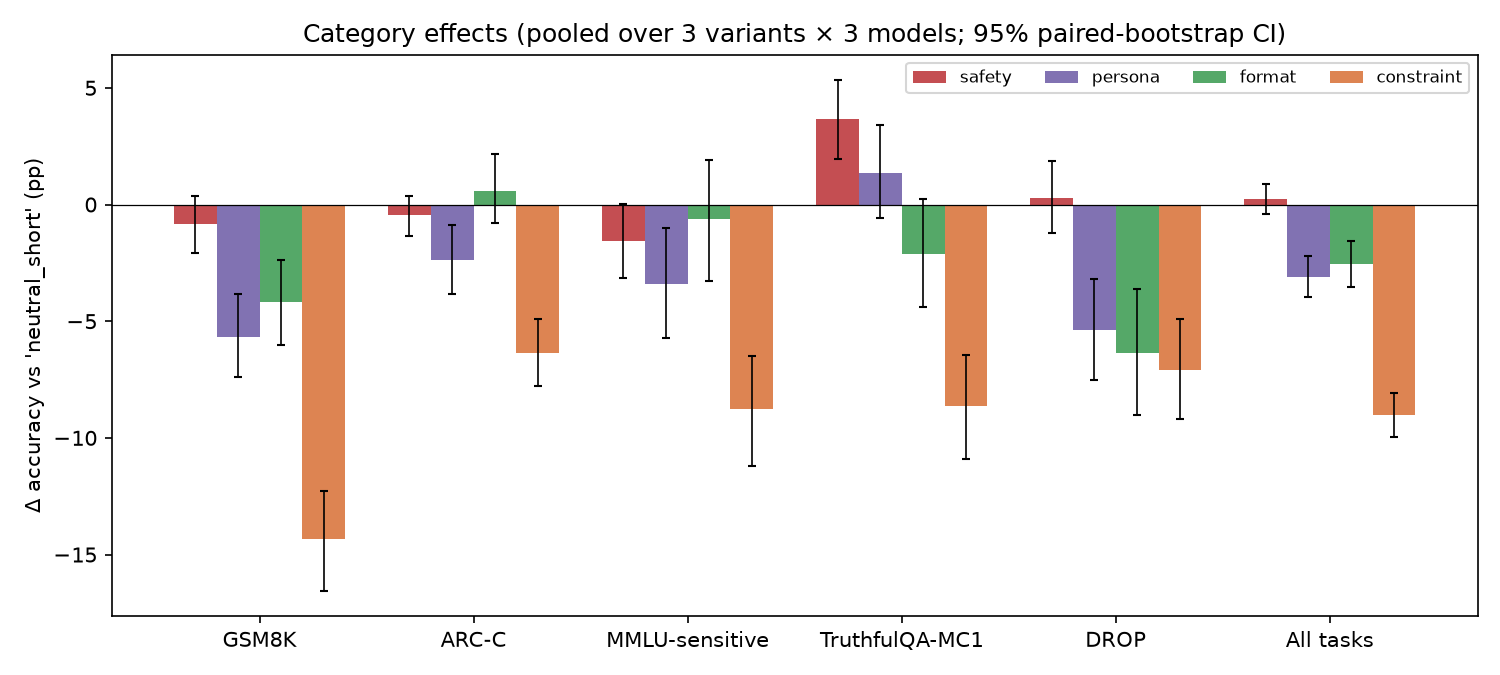
\includegraphics[width=0.95\linewidth]{figures/category_effects_greedy_correct_lenient.png}
\caption{Lenient accuracy change by category and task, pooled over three variants and three models (error bars: 95\% paired-bootstrap CI). \safety is indistinguishable from zero everywhere except \tqa, where it helps. \constraint is the most harmful category on every task, with the largest loss on \gsm ($-14.3$\pp).}
\label{fig:category}
\end{figure}

\subsection{Main result: which categories cost accuracy?}
\label{sec:main}

\Tabref{tab:main} and \figref{fig:category} give the category effects.

{\bf Safety prompts are nearly free.} The pooled \safety effect is $+0.2$\pp (95\% CI $[-0.4, 0.9]$). No task shows a significant loss, and \tqa shows a significant {\em gain} of $+3.7$\pp. This contradicts H1, which predicted a 4--8\pp loss.

{\bf Personas cost accuracy and double length.} \persona prompts lower accuracy by 3.1\pp, with significant losses on four of five tasks (up to $-5.7$\pp on \gsm). They roughly double output length ($1.99\times$), far above the 30--50\% predicted by H2.

{\bf Format prompts do not make answers more correct.} Under lenient scoring, \format lowers accuracy by 2.5\pp, with significant losses on \gsm ($-4.2$\pp) and \drop ($-6.4$\pp). On the structured tasks the hypothesis targeted, the effect is $-2.1$\pp, not $+2$--$5$\pp.

{\bf Constraints are the most harmful.} \constraint prompts lower accuracy by 9.0\pp, with significant losses on every task and the largest on \gsm ($-14.3$\pp). They also shorten outputs to $0.41\times$ the baseline length.

{\bf The controls barely move accuracy.} Removing the system prompt costs $-0.5$\pp (CI includes zero), and the length-matched \neutrallong blurb costs $-1.4$\pp. Because \neutrallong is as long as the category prompts but much less harmful than \persona or \constraint, the larger effects come from what the prompts {\em say}, not from how long they are.

\subsection{Strict scoring: parseability is a different story}
\label{sec:strict}

The lower half of \tabref{tab:main} uses a strict parser that only accepts explicit answer markers. The picture reverses for format prompts. \format is now the only helpful category, at $+19.6$\pp overall and $+58.1$\pp on \drop, because format prompts produce an explicit marker in 99.5\% of responses, compared with 73\% at baseline. \safety drops to $-4.4$\pp under strict scoring, because safety-prompted answers use an explicit marker less often (63--68\% \versus 73\%). This is a parsing effect, not a reasoning effect: the same answers score $+0.2$\pp under lenient scoring. \persona ($-14.8$\pp) and \constraint ($-44.8$\pp) lose far more under strict scoring, since chatty prose and brevity both tend to drop answer markers. Which scorer matters depends on the deployment: a pipeline that reads a JSON field sees the strict numbers, while a human reader sees something closer to the lenient numbers.

\subsection{Effects depend on the model}
\label{sec:per_model}

\begin{table}[t]
\centering
\resizebox{\textwidth}{!}{%
\begin{tabular}{@{}lcccccc@{}}
\toprule
& \multicolumn{3}{c}{\textbf{Lenient $\Delta$ (pp)}} & \multicolumn{3}{c}{\textbf{Length ratio}} \\
\cmidrule(lr){2-4} \cmidrule(lr){5-7}
\textbf{Category} & \llama & \qwentwo & \qwenthree & \llama & \qwentwo & \qwenthree \\
\midrule
\safety     & $-$0.7 & +0.3 & {\bf +1.1} & 1.19$\times$ & 1.04$\times$ & 1.04$\times$ \\
\persona    & $-$4.4 & $-$5.1 & {\bf +0.2} & 2.10$\times$ & 1.76$\times$ & 2.11$\times$ \\
\format     & $-$4.1 & $-$3.7 & {\bf +0.2} & 1.14$\times$ & 0.82$\times$ & 0.94$\times$ \\
\constraint & {\bf $-$4.6} & $-$14.2 & $-$8.2 & 0.55$\times$ & 0.33$\times$ & 0.37$\times$ \\
\bottomrule
\end{tabular}}
\caption{Per-model category effects (greedy, lenient, mean over tasks and variants) and output-length ratios relative to \baseline. The most robust model in each row is in \textbf{bold}. \qwenthree is unaffected by personas and format prompts, but still loses 8.2\pp under constraints; \qwentwo is hurt most by constraints.}
\label{tab:per_model}
\end{table}


\Tabref{tab:per_model} breaks the category effects down by model. \qwenthree, the newest model, is robust to personas ($+0.2$\pp) and format prompts ($+0.2$\pp), while \llama and \qwentwo lose 3.7 to 5.1\pp under both. All three models still lose under constraints, with \qwentwo hurt most ($-14.2$\pp). The persona length effect, by contrast, appears in all three models ($1.76$--$2.11\times$). Residual effects on accuracy are therefore partly a property of a model's instruction tuning, while the length effect is more universal.

\subsection{Output length}
\label{sec:length}

\begin{figure}[t]
\centering
\begin{subfigure}[b]{0.48\textwidth}
    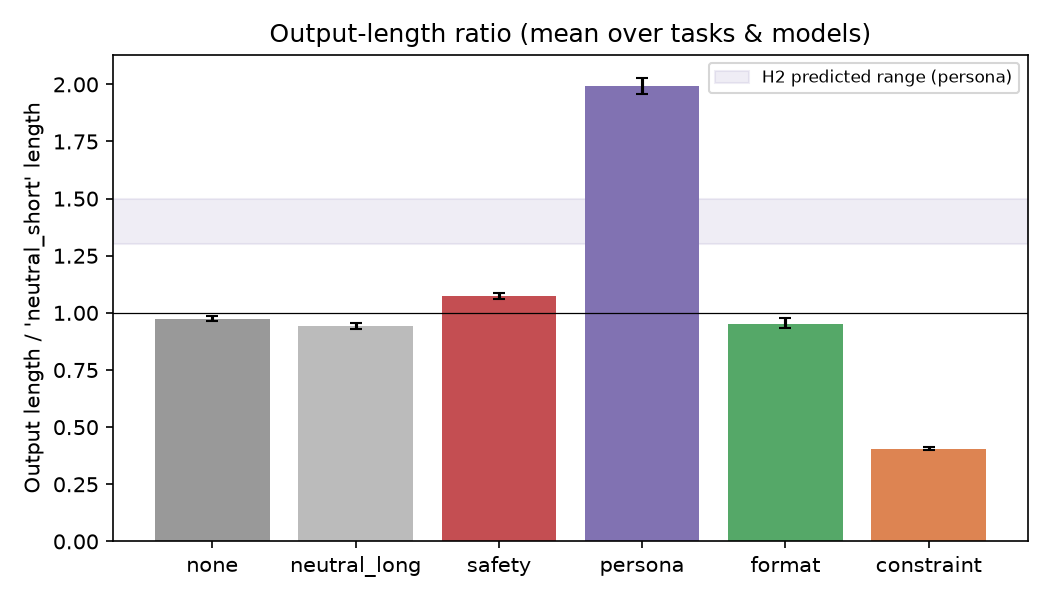
\includegraphics[width=\textwidth]{figures/length_ratio_greedy.png}
    \caption{Output-length ratio \versus \baseline}
    \label{fig:length}
\end{subfigure}
\hfill
\begin{subfigure}[b]{0.48\textwidth}
    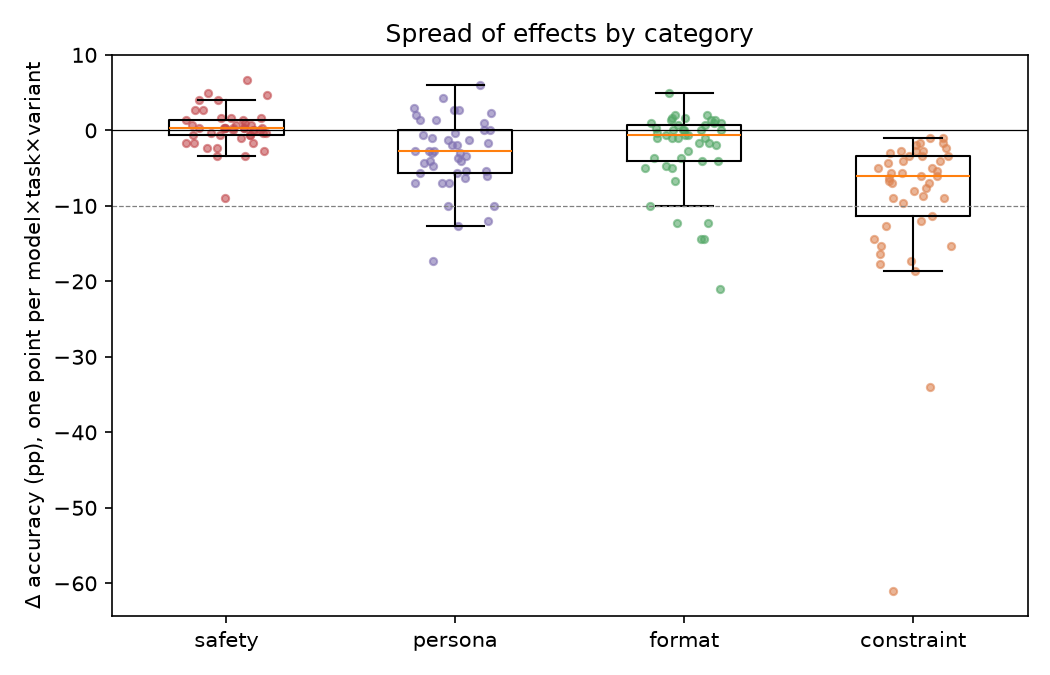
\includegraphics[width=\textwidth]{figures/effect_spread_greedy_correct_lenient.png}
    \caption{Spread of cell-level accuracy effects}
    \label{fig:spread}
\end{subfigure}
\caption{\captiona Mean output length relative to \baseline (error bars: 95\% CI). Personas double length, far beyond the range predicted by H2 (shaded), while the length-matched \neutrallong control does not lengthen outputs. \captionb Lenient accuracy change for each of the 45 model $\times$ task $\times$ variant cells per category. \constraint has by far the widest spread, but it lies entirely below zero; the dashed line marks $-10$\pp.}
\label{fig:length_spread}
\end{figure}

\Figref{fig:length} shows the length ratios. Personas produce about $2\times$ longer outputs, with per-cell ratios from $0.89\times$ (\qwentwo on \gsm) to $3.4\times$; on MC tasks the ratio is $1.8$--$2.6\times$. Safety prompts add 7\%. Format prompts shorten outputs by 5\% on average, but this hides large differences between variants: JSON output is much shorter ($0.65\times$ on \gsm), while the \texttt{Final Answer} format is slightly longer than baseline. Constraints cut length by 59\%. The \neutrallong control does not lengthen outputs ($0.94\times$), so the persona length effect comes from persona content, not from prompt length.

\subsection{Hedging and refusal}
\label{sec:hedge}

\begin{table}[t]
\centering
\small
\begin{tabular}{@{}lccc@{}}
\toprule
\textbf{Condition} & \textbf{Refusal / clarif.\ (\%)} & \textbf{Hedge / caveat (\%)} & \textbf{Unparseable (\%)} \\
\midrule
\baseline & 0.2 & 1.4 & 0.2 \\
\neutrallong & {\bf 1.1} & 1.7 & 1.2 \\
\midrule
\cond{safety\_A / B / C} & 0.3 / 0.6 / 1.0 & {\bf 7.2} / 4.0 / 2.5 & 0.9 / 1.0 / 0.8 \\
\cond{persona\_A / B / C} & 0.1 / 0.5 / 0.1 & 3.8 / 2.5 / 3.6 & 1.9 / 1.2 / 1.2 \\
\cond{format\_A / B / C} & $\le$0.2 & $\le$0.5 & $\le$0.3 \\
\cond{constraint\_A / B / C} & 0.0 & 0.0 / 1.6 / 0.1 & 0.3 / {\bf 7.4} / 2.9 \\
\bottomrule
\end{tabular}
\caption{Response behaviour by condition (greedy, all tasks and models; 4,500 responses per condition). The highest value in each column is in \textbf{bold}. Safety prompts raise hedging up to $5\times$ the baseline rate, yet refusals stay at or below 1\% in every condition. The highest refusal rate comes from the behaviourally empty \neutrallong blurb.}
\label{tab:behaviour}
\end{table}


\Tabref{tab:behaviour} and \figref{fig:hedge} (appendix) report response behaviour. Safety prompts raise the rate of hedging and caveat phrases from 1.4\% to as much as 7.2\% (\cond{safety\_A}), but refusals stay at or below 1.0\%. Almost all refusals under safety prompts come from \llama, for example ``I cannot provide information that could be used to harm the environment'' on an ARC ecology question. The models thus treat safety text mainly as a tone instruction: they add disclaimers but still commit to an answer.

{\bf A surprise: scope refusals from a neutral blurb.} The behaviourally empty \neutrallong control produces the highest refusal rate (1.1\%). \llama refuses 3.1\% of questions under this prompt with replies such as ``I can't answer that question as it is not related to the Northwind Learning Hub''. Neither Qwen model does this. A deployment description, with no instruction to stay on topic, is enough to make one model restrict its own scope.

\subsection{How items flip from right to wrong}
\label{sec:flips}

\begin{table}[t]
\centering
\resizebox{\textwidth}{!}{%
\begin{tabular}{@{}lccccccc@{}}
\toprule
& \multicolumn{3}{c}{\textbf{Flips}} & \multicolumn{4}{c}{\textbf{Right $\to$ wrong, by failure type}} \\
\cmidrule(lr){2-4} \cmidrule(lr){5-8}
\textbf{Condition} & Right$\to$wrong & Wrong$\to$right & Net (pp) & Refusal & Unparseable & Hedged-wrong & Plain wrong \\
\midrule
\cond{safety\_A}      & 162 & 180 & {\bf +0.4} & 2 & 17 & 21 & 122 \\
\cond{safety\_B}      & 162 & 176 & +0.3 & 6 & 12 & 9 & 135 \\
\cond{persona\_A}     & 450 & 258 & $-$4.3 & 1 & 53 & 14 & 382 \\
\cond{format\_C} (JSON) & 441 & 264 & $-$3.9 & 1 & 2 & 1 & 437 \\
\cond{constraint\_A}  & 544 & 157 & $-$8.6 & 1 & 3 & 0 & 540 \\
\cond{constraint\_B}  & 593 & 187 & $-$9.0 & 0 & {\bf 223} & 10 & 360 \\
\bottomrule
\end{tabular}}
\caption{How items flip relative to \baseline for selected conditions (greedy; 4,500 item--model pairs per condition). Safety losses are balanced by gains, and refusal is never a meaningful failure mode. Most losses are plain wrong answers, except under \cond{constraint\_B}, where over a third of losses are answers the scorer cannot map to an option.}
\label{tab:flips}
\end{table}


\begin{figure}[t]
\centering
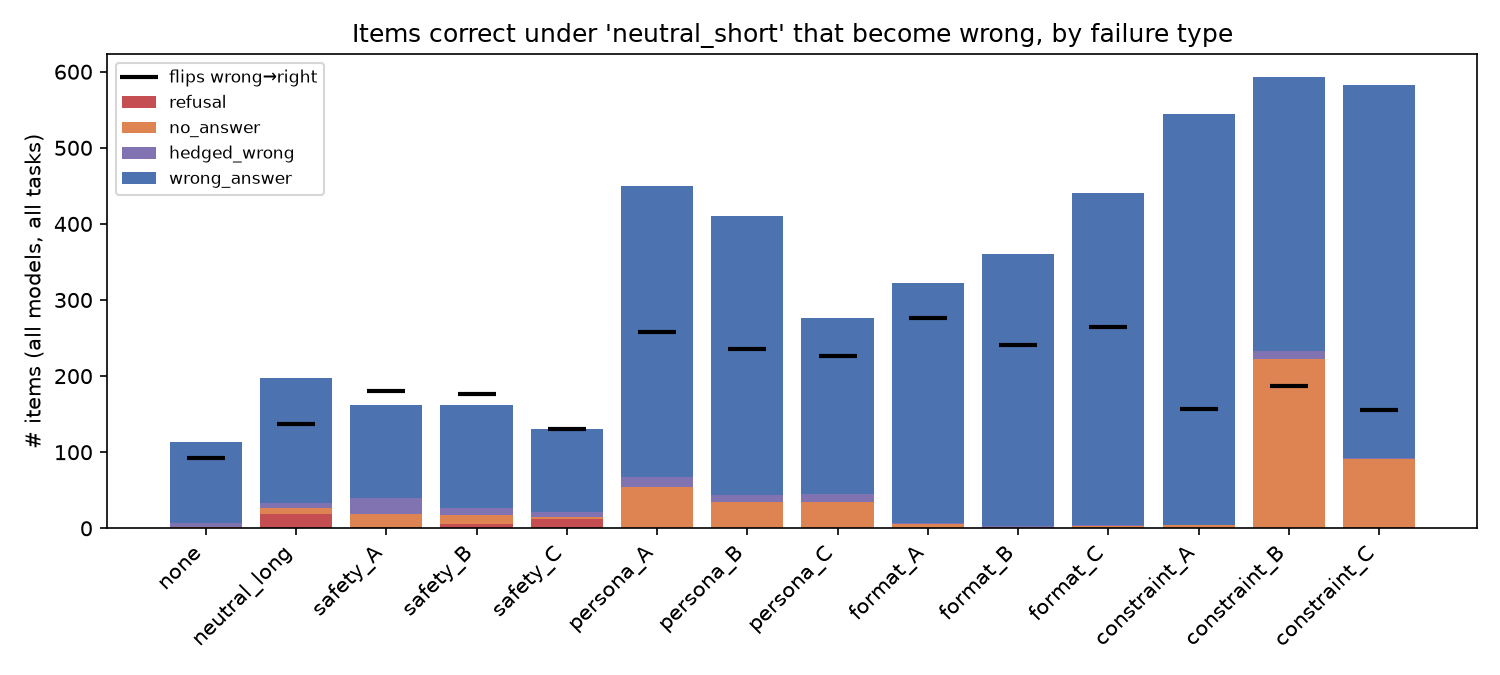
\includegraphics[width=0.95\linewidth]{figures/flip_types.png}
\caption{Items correct under \baseline that become wrong under each condition, split by failure type (all models and tasks). Black bars mark the reverse flips (wrong $\to$ right). For safety prompts the two directions are balanced. For persona, format and constraint prompts, losses greatly exceed gains, and most losses are plain wrong answers rather than refusals or parse failures.}
\label{fig:flips}
\end{figure}

\Tabref{tab:flips} and \figref{fig:flips} decompose the losses. We read failing responses for each category and find distinct mechanisms.

\para{Safety: balanced churn.} \cond{safety\_A} turns 162 correct items wrong but 180 wrong items right. Refusals account for only 2 of the 162 losses.

\para{Persona: lost focus.} Persona responses contain digressions and anecdotes, and some end without committing to an answer (``\ldots Isn't it fascinating\ldots?''). Most losses are plain wrong answers (382 of 450 for \cond{persona\_A}), with a smaller share of unparseable responses (53).

\para{Format: compressed reasoning and rule spill-over.} JSON and markdown-section formats compress the reasoning into a plan without carrying out the arithmetic. For example, under \cond{format\_B} one \gsm response listed four reasoning bullets (``Subtract \ldots\ to find the leftover money'') and then answered \texttt{\#\# Answer 100000} (gold: 40000). \cond{format\_C} (JSON) costs 10.1\pp on \gsm. A second failure is rule spill-over: \cond{format\_A} says that ``for multiple-choice questions the final answer must be the single letter''. \qwentwo applies this rule to \drop, which has no options, in 18\% of its answers, writing ``Final Answer: R'' for {\em Republican} and ``J'' for {\em Jeff Garcia}.

\para{Constraint: removed reasoning and unscorable prose.} \cond{constraint\_A} (``under 50 words, don't show intermediate work'') removes chain-of-thought. For \qwentwo on \gsm this costs 61\pp, the largest cell-level effect in the study. \cond{constraint\_B} (``plain prose only'') leads models to paraphrase an option without naming its letter; 223 of its 593 losses are unparseable (7--16\% of MC answers). Even after accounting for these, it still lowers content accuracy.

\subsection{Dispersion of constraint effects (H4)}
\label{sec:dispersion}

H4 predicted that constraints would have the most variable effects, helping some tasks and hurting others by at least 10\pp. \Figref{fig:spread} shows that constraints do have by far the widest cell-level spread: an SD of 10.1\pp across the 45 cells, compared with 2.5 (\safety), 4.7 (\persona) and 5.2\pp (\format). Twelve of 45 constraint cells are at or below $-10$\pp, and the minimum is $-61$\pp. However, the across-task SD of the pooled effect (3.1\pp, CI $[2.4, 4.3]$) is not distinguishable from persona (2.8) or format (2.8), whose CIs overlap. Most importantly, constraints never help: the best constraint cell is $-1.0$\pp, and none of the 45 cells is significantly positive (34 are significantly negative). The variance is between ``hurts a little'' and ``hurts badly'', not between helping and hurting.

\subsection{Robustness}
\label{sec:robustness}

\para{Answered-only accuracy.} If we keep only items where an answer was extracted under both baseline and condition, the ordering of categories is unchanged: \safety $+0.5$, \persona $-2.3$, \format $-2.6$ and \constraint $-6.9$\pp. Parse failures explain part of the persona and constraint losses, but not all of them.

\para{Prompt length.} The length-matched \neutrallong control costs only $-1.4$\pp, much less than \persona ($-3.1$) or \constraint ($-9.0$), whose prompts are of similar or shorter length.

\begin{figure}[t]
\centering
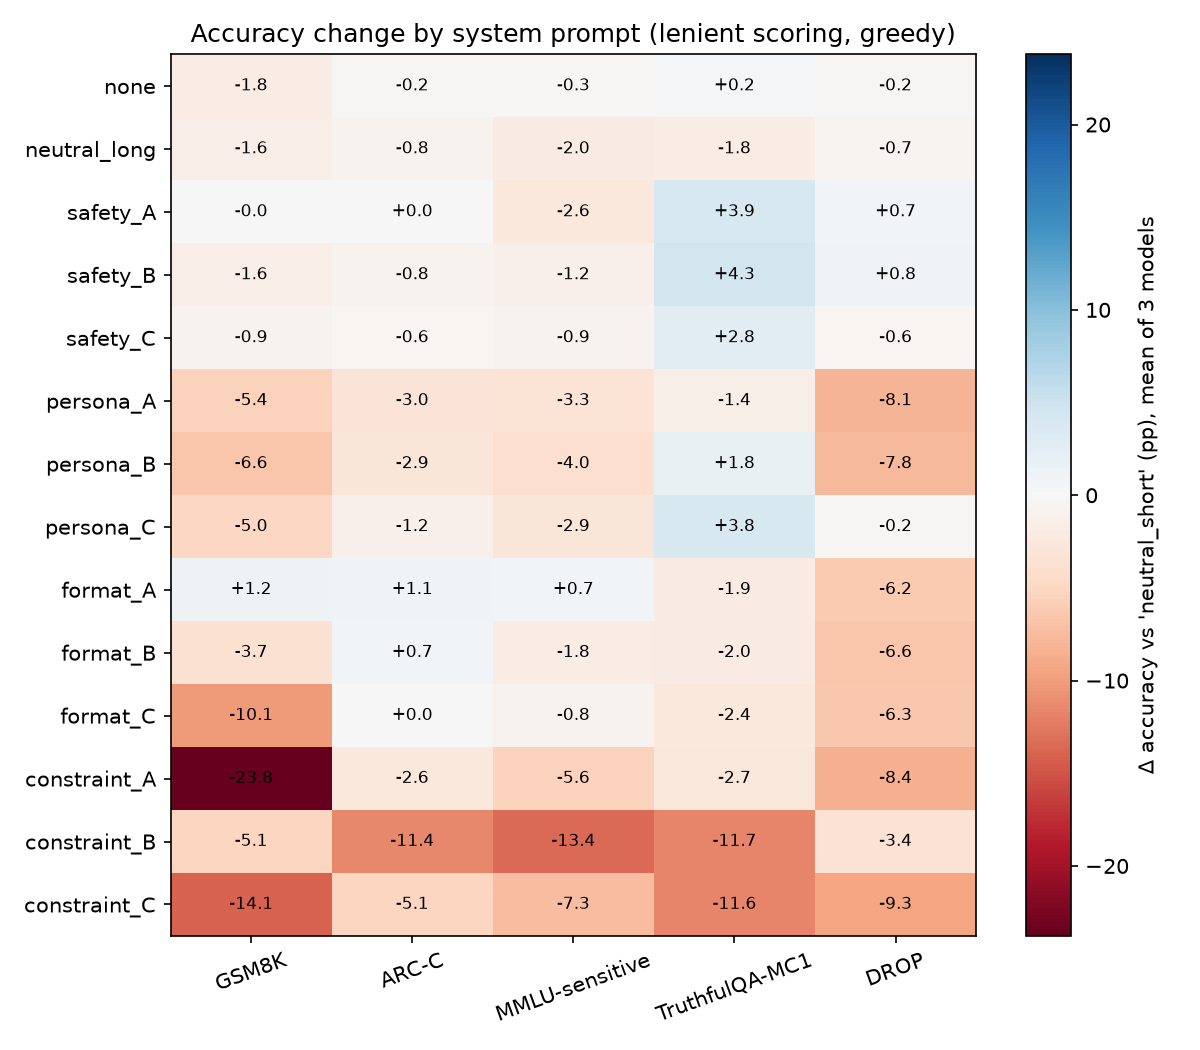
\includegraphics[width=0.62\linewidth]{figures/heatmap_delta_greedy_correct_lenient.png}
\caption{Lenient accuracy change (pp) for every condition and task, averaged over three models. Safety variants agree closely, and all three improve \tqa. Format and persona effects depend strongly on wording: \cond{format\_A} is slightly positive on \gsm, \arc and \mmlus, while \cond{format\_C} (JSON) loses 10.1\pp on \gsm, and \cond{persona\_C} is far less harmful than \cond{persona\_A} and \cond{persona\_B}.}
\label{fig:heatmap}
\end{figure}

\para{Wording variants.} \Figref{fig:heatmap} shows each condition separately. The three safety variants all improve \tqa ($+2.8$ to $+4.3$\pp) and stay within $\pm2.6$\pp of baseline on every other task; they disagree in sign only on \drop ($+0.7$, $+0.8$, $-0.6$). Format variants differ much more: \cond{format\_A} is slightly positive on \gsm, \arc and \mmlus ($+0.7$ to $+1.2$\pp) but loses 1.9\pp on \tqa and 6.2\pp on \drop, while \cond{format\_C} loses 10.1\pp on \gsm. {\em Which} format is requested matters more than whether a format is requested. Among personas, the ``thorough consultant'' (\cond{persona\_C}) is much less harmful than the lecturer and the comedian.

\para{Sensitive MMLU subjects.} Within \mmlus, the largest safety loss is on moral scenarios ($-8.3$\pp over 59 items $\times$ 3 models), which is consistent with caution on morally loaded judgments. Medical subjects change by $-5.6$ to $+3.7$\pp, but with only 5--19 items per subject, no per-subject result is conclusive.

\begin{table}[t]
\centering
\resizebox{\textwidth}{!}{%
\begin{tabular}{@{}lccccc@{}}
\toprule
& \multicolumn{2}{c}{\textbf{Lenient $\Delta$ (pp)}} & \multicolumn{2}{c}{\textbf{Strict $\Delta$ (pp)}} & \textbf{Length ratio} \\
\cmidrule(lr){2-3} \cmidrule(lr){4-5} \cmidrule(lr){6-6}
\textbf{Category} & Greedy & $T{=}0.7$ & Greedy & $T{=}0.7$ & Greedy / $T{=}0.7$ \\
\midrule
\safety     & {\bf +0.2} \ci{$-$0.4}{0.9} & {\bf +0.4} \ci{$-$0.3}{1.1} & $-$4.4 & $-$5.1 & 1.07$\times$ / 1.07$\times$ \\
\persona    & $-$3.1 \ci{$-$4.0}{$-$2.2} & $-$2.8 \ci{$-$3.6}{$-$1.9} & $-$14.8 & $-$15.2 & 1.99$\times$ / 1.99$\times$ \\
\format     & $-$2.5 \ci{$-$3.6}{$-$1.6} & $-$2.0 \ci{$-$2.9}{$-$1.0} & {\bf +19.6} & {\bf +20.2} & 0.95$\times$ / 0.94$\times$ \\
\constraint & $-$9.0 \ci{$-$10.0}{$-$8.1} & $-$8.7 \ci{$-$9.7}{$-$7.7} & $-$44.8 & $-$44.8 & 0.41$\times$ / 0.41$\times$ \\
\textit{Control:} \neutrallong & $-$1.4 & $-$1.1 & -- & -- & 0.94$\times$ / 0.95$\times$ \\
\bottomrule
\end{tabular}}
\caption{Greedy decoding \versus a full temperature-0.7 sampling replicate (top-$p$ 0.95; 67,500 generations each), pooled over models and tasks, with 95\% CIs. Best category per column in \textbf{bold}. Category-level effects move by at most 0.6\pp (lenient) and 0.7\pp (strict).}
\label{tab:replicate}
\end{table}


\para{Sampling replicate.} We rerun the entire grid at temperature 0.7 (\tabref{tab:replicate}). For \qwenthree, this replicate also switches from FP8 to bf16 weights, so it tests robustness to quantisation as well. Category effects move by at most 0.6\pp (lenient) and 0.7\pp (strict), and every hypothesis verdict is unchanged. Across the 210 non-baseline cells, greedy and sampled effects correlate strongly (Pearson $r=0.95$, Spearman $\rho=0.87$; per model $r=0.84$, $0.98$ and $0.93$ for \llama, \qwentwo and \qwenthree), with a mean absolute difference of 1.7\pp. Of the 63 cells significant under greedy decoding (McNemar $p<0.05$), 98\% keep their sign and 81\% are again significant with the same sign. Overall sign agreement is only 76\%, but the disagreements come from cells near zero: for cells with $|\Delta|<2$\pp, signs agree only 59\% of the time, close to chance. Small per-cell effects should therefore be read as noise. Task-level patterns also replicate: safety again improves \tqa ($+4.4$\pp, Holm $p<0.05$), constraints again are worst on every task (\gsm $-13.7$\pp), and \constraint again has the widest cell-level spread (SD 10.8 \versus 2.9--5.5\pp) with no significantly positive cell. Behaviour replicates too: \cond{safety\_A} hedges in 6.8\% of responses (baseline 1.3\%), refusals stay at or below 0.9\%, and format prompts yield explicit answer markers in 99.4--99.8\% of responses \versus 71.7\% at baseline.

\subsection{Summary of hypotheses}

\begin{table}[t]
\centering
\small
\renewcommand{\arraystretch}{1.2}
\begin{tabular}{@{}p{3.6cm}p{2.3cm}p{7.2cm}@{}}
\toprule
\textbf{Hypothesis} & \textbf{Verdict} & \textbf{Evidence} \\
\midrule
H1: \safety costs 4--8\pp via hedging and refusal & Not supported & Lenient $\Delta=+0.2$ \ci{$-$0.4}{0.9}; \tqa $+3.7$\pp. Hedging rises (1.4\%$\to$7.2\%), refusals $\le$1\%. The $-4.4$\pp strict loss comes from fewer explicit answer markers, not worse reasoning. \\
H2: \persona adds 30--50\% length, no gain & Direction yes, magnitude no & Length $1.99\times$ \ci{1.96}{2.03}; accuracy does not improve and drops by 3.1\pp. \\
H3: \format is the only helpful category (+2--5\pp) & Supported only for parseability & Lenient $\Delta=-2.5$ (\gsm $-4.2$, \drop $-6.4$); strict $\Delta=+19.6$. \safety, not \format, is the only category with a non-negative content effect. \\
H4: \constraint has the largest variance, helps some tasks, hurts others by $\ge$10\pp & Partly supported & Largest cell-level SD (10.1 \versus 2.5--5.3\pp), 12/45 cells $\le-10$\pp, minimum $-61$\pp. Across-task SD (3.1) overlaps persona/format (2.8). Never helps: best cell $-1.0$\pp, 0/45 significantly positive. \\
\bottomrule
\end{tabular}
\caption{Verdicts for the four hypotheses (greedy decoding; all verdicts are unchanged under $T{=}0.7$).}
\label{tab:hypotheses}
\end{table}


\Tabref{tab:hypotheses} summarizes the verdicts. Two of the four hypotheses are not supported for content accuracy (H1, H3), and the other two are supported only in part (H2, H4). The common pattern is that the expected {\em costs} of safety text are absent, while the costs of personas and constraints are larger or more one-sided than expected.
